\documentclass{article}
\usepackage{doc,url,verbatim,fancyvrb}
\usepackage{pifont}
\usepackage[authoryear]{natbib}
\usepackage[pdftex]{graphicx}
\usepackage{gretl}
\usepackage[letterpaper,body={6.3in,9.15in},top=.8in,left=1.1in]{geometry}
\usepackage[pdftex,hyperfootnotes=false]{hyperref}

% \usepackage[a4paper,body={6.1in,9.7in},top=.8in,left=1.1in]{geometry}

\begin{document}

\setlength{\parindent}{0pt}
\setlength{\parskip}{1ex}
\setcounter{secnumdepth}{1}

% \newenvironment{funcdoc}[1]
% {\noindent\hrulefill\newline\texttt{#1}\par\noindent\hrulefill\par\medskip\par}
% {\bigskip}

\newenvironment{funcdoc}
{\noindent\hrulefill\\[-10pt]}
{\medskip}

\newcommand{\argname}[1]{\textsl{#1}}

\title{dbnomics for gretl, version 0.1}
\author{Jack Lucchetti \and Allin Cottrell}
\maketitle

\section{Introduction}

This package offers an interface to \textsf{dbnomics} for gretl. For
anyone who hasn't yet caught on, \textsf{dbnomics} makes available, in
a uniform manner, a huge number of macroeconomic data series drawn
from many sources around the world---a truly admirable service!

There are at present two variants of the \textsf{dbnomics} site: the
original version at \url{https://db.nomics.world/} and the new or
``next'' version at \url{https://next.nomics.world/}. This package
targets the ``next'' version, which encompasses many more data
providers than the original. Interested users are encouraged to visit
the site to get a better sense of what's available.  But please note:
the new version is still work in progress, which means that some
aspects of this package are likely to change as bugs are discovered
and fixed at \textsf{dbnomics}. We will endeavor to keep our package
up to date and will push out any updates with gretl snapshots.

There are three main layers to the \textsf{dbnomics} ``space,'' as
follows:
\begin{itemize}
\item \textit{Providers}: the various statistical agencies that are
  the primary sources of the data. As of this writing 31 providers
  are included.
\item \textit{Datasets}: sets of related series offered by a given
  provider. Over 8000 datasets are available.
\item \textit{Series}: specific time series such as the Bulgarian
  unemployment rate. Hundreds of millions of series are available.
\end{itemize}

A specific series in \textsf{dbnomics} is identified by a triplet
of the form \texttt{provider/dataset/series}, for example
\begin{code}
ECB/IRS/M.IT.L.L40.CI.0000.EUR.N.Z
\end{code}
Here the provider is \texttt{ECB} (the European Central Bank); the
dataset is \texttt{IRS} (interest rate statistics); and the particular
series is ``\texttt{M.IT.L.L40.CI.0000.EUR.N.Z},'' an Italian 10-year
interest rate.

This package provides means of downloading a specific series if you
know its identifying triplet, and also means of navigating the
\textsf{dbnomics} space. There are three ways of accessing the
functionality of the package:
\begin{itemize}
\item Via the gretl commands \cmd{open} and \cmd{data}, as with native
  gretl databases.
\item By means of the gretl GUI.
\item By calling the public functions of the package yourself, in
  command-line or scripting mode.
\end{itemize}
The following three sections expand on these methods in turn.

\section{The \texttt{open} and \texttt{data} commands}
\label{sec:open-data}

To exploit this method you need to know the identifying triplet(s) for
the series you want. Given that, you can initiate \textsf{dbnomics}
access via the command
\begin{code}
open dbnomics
\end{code}
From this point the \cmd{data} command will target \textsf{dbnomics}
data until you ``\texttt{open}'' some other data source. So, for
example, you could download the Italian 10-year interest rate
mentioned above in this way:
\begin{code}
data ECB/IRS/M.IT.L.L40.CI.0000.EUR.N.Z
\end{code}
Ah, but what about the name of the series within gretl? The full
triplet is obviously not acceptable as a gretl series-name, and even
its third component won't work since gretl identifiers cannot contain
the dot character. What happens by default is that gretl takes the
third portion of the triplet and squeezes out any illegal characters.
In the case above this would give a name of
\texttt{MITLL40CI0000EURNZ}---not very nice-looking. However, you can
take charge of the naming of the imported series yourself, using the
\option{name} option to the \cmd{data} command, as in
\begin{code}
data ECB/IRS/M.IT.L.L40.CI.0000.EUR.N.Z --name="IT_10yr"
\end{code}
In this case the series will be known to gretl as \texttt{IT\_10yr}.
Note that when you import a series from \textsf{dbnomics} its
descriptive ``label'' starts with the full triplet so you won't lose
that information of record, regardless of the naming of the series.

\section{dbnomics via the gretl GUI}
\label{sec:dbn-gui}

GUI access to \textsf{dbnomics} is provided in two places (see
Figures~\ref{fig:db-access-1} and \ref{fig:db-access-2}):
\begin{itemize}
\item Via the \textsf{Databases} item under the \textsf{File} menu in
  the gretl main window.
\item From the gretl databases window (opened by the database icon on
  the toolbar at the foot of the main window): click the ``DB'' icon
  on the toolbar in this window.
\end{itemize}

\begin{figure}[htbp]
  \centering
  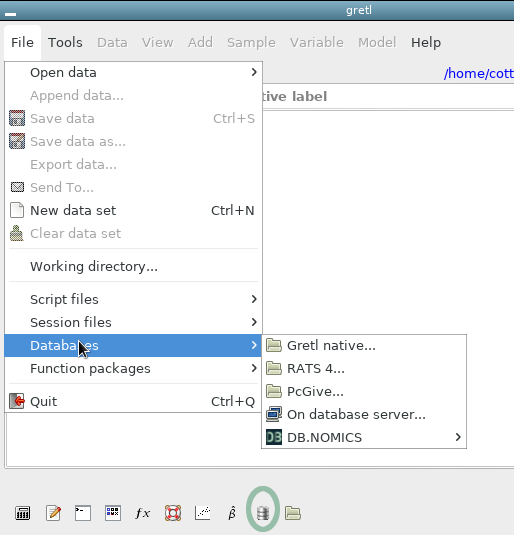
\includegraphics[scale=2.0]{db-access-1}
  \caption{DB.NOMICS access via the File menu or the databases
    button (circled)}
  \label{fig:db-access-1}
\end{figure}

\begin{figure}[htbp]
  \centering
  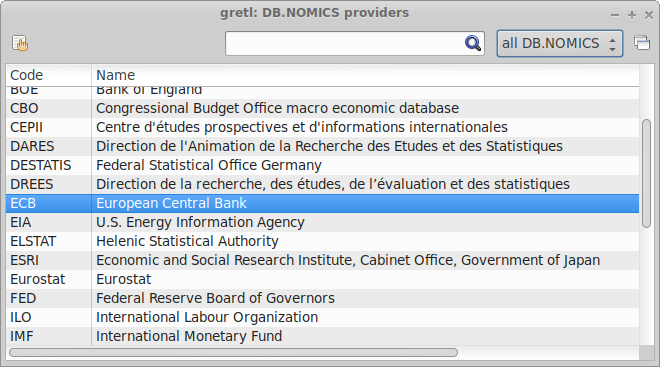
\includegraphics[scale=0.5]{db-access-2}
  \caption{The DB.NOMICS button in the primary databases window}
  \label{fig:db-access-2}
\end{figure}

In both cases you get a little sub-menu with entries
``\textsf{Browse}'' and ``\textsf{Specific series}.'' The latter entry
takes you to a dialog box in which you can enter a series triplet (see
section~\ref{sec:open-data}). The \textsf{Browse} entry takes you to a
window which displays the available \textsf{dbnomics} providers: their
codes and their descriptions. From here you have two options:
\begin{itemize}
\item Select a provider and double-click to browse the datasets it
  supplies.
\item In the search box in the top panel of the window, enter a string
  and search all providers for datasets that match your
  specification.\footnote{If you wish to use this facility to find a
    string in the providers window itself, first select ``\textsf{this
      window}'' to the right of the search box, the default being
    ``\textsf{all DB.NOMICS}.''}
\end{itemize}

In each case a \textsf{dbnomics} datasets window will open. With some
providers or searches more datasets will be found than can comfortably
be displayed at once. In that case the toolbar includes buttons that
let you page forward or back through the listing; you should also get
a status message at the foot of the window indicating the current
position in the listing.

From a datasets window two more steps are available:
\begin{itemize}
\item Double-click on a dataset to open a window showing the series it
  contains (or one ``page'' of its full list of series if there are
  too many).
\item In a window showing \textsf{dbnomics} series, double-click to
  activate a particular series. This will give you detailed
  information on the series and allow you to display its values,
  create a time-series plot, or add the series to your gretl dataset.
\end{itemize}

To summarize, there are three layers to gretl's GUI representation of
the \textsf{dbnomics} space:
\begin{enumerate}
\item The providers window
\item Datasets window (for a given provider, or via search)
\item Series window (for a given dataset)
\end{enumerate}

\section{Public functions}
\label{sec:dbn-funcs}

The package contains several public functions which both subserve the
modes of access described in sections~\ref{sec:open-data} and
\ref{sec:dbn-gui}, and can be called directly by the user.

At this point we just offer an ``as is'' listing of the signatures of
these functions with brief commentary. The finer points are subject to
change; we can expand on them later if there's sufficient
interest. Note that this package contains several test scripts that
exemplify calls to the functions listed below; this can be found in
the \texttt{examples} subdirectory of the installation
directory. Likely locations for this are as follows (though the paths
may differ by locale and otherwise):

{\small
\begin{tabular}{ll}
  Linux & \texttt{/usr/share/gretl/functions/dbnomics} \\
  Windows & \verb|C:\Program Files\gretl\functions\dbnomics| \\
  Mac & \texttt{/Applications/Gretl.app/Contents/Resources/share/gretl/functions/dbnomics}
\end{tabular}
}

\bigskip

\begin{funcdoc}
\begin{verbatim}
bundles dbnomics_providers (bool verbose[0])
\end{verbatim}
Returns an array of bundles, one per provider. Each bundle contains
basic info about the provider, notably its dbnomics code under the
\texttt{code} key and its full name under the \texttt{name} key.
\end{funcdoc}

\begin{funcdoc}
\begin{verbatim}
bundle dbnomics_dsets_for_provider (const string provider,
                                    bool verbose[0])
\end{verbatim}
  Returns a bundle containing basic information on the datasets
  associated with a given provider, namely two arrays of strings
  holding the codes and names of the datasets respectively.
\begin{code}
# example
bundle b = dbnomics_dsets_for_provider("AMECO")
\end{code}
\end{funcdoc}

\begin{funcdoc}
\begin{verbatim}
bundles dbnomics_get_dataset_content (const string provider,
                                      const string dset,
                                      int limit[0::100],
                                      int offset[0])
\end{verbatim}
Returns an array of bundles each containing information on a series
contained in the dataset specified by the \texttt{provider} and
\texttt{dset} codes. The \texttt{limit} and \texttt{offset}
arguments allow ``paging'': retrieve so many results, starting at a
given offset into the full listing.
\begin{code}
# example
bundles B = dbnomics_get_dataset_content("ECB", "IRS", 50, 100)
\end{code}
\end{funcdoc}

\begin{funcdoc}
\begin{verbatim}
bundle dbnomics_get_series (const string datacode,
                            bool verbose[0],
                            string *from_json[null])
\end{verbatim}
Returns a bundle containing information on the series specified by
\texttt{datacode}, which must be a \textsf{dbnomics} triplet as
described above.
\begin{code}
# example
bundle b = dbnomics_get_series("ECB/IRS/M.IT.L.L40.CI.0000.EUR.N.Z")
\end{code}
\end{funcdoc}

\begin{funcdoc}
\begin{verbatim}
void dbnomics_bundle_print (const bundle b,
                            bool print_data[0])
\end{verbatim}
Displays the content of a bundle obtained by
\texttt{dbnomics\_get\_series}. Give a non-zero value for the second
argument to print the actual values, otherwise just the metadata is
shown.
\end{funcdoc}

\begin{funcdoc}
\begin{verbatim}
scalar dbnomics_bundle_get_data (const bundle b,
                                 series *x,
                                 bool verbose[0])
\end{verbatim}
Given a bundle obtained by \texttt{dbnomics\_get\_series}, writes the
actual data values (and description) into the series \texttt{x}, which
must exist already and be given in ``pointer'' form. Returns zero on
success, non-zero on error.
\begin{code}
# example
bundle b = dbnomics_get_series("ECB/IRS/M.IT.L.L40.CI.0000.EUR.N.Z")
series IT_10yr = NA
dbnomics_bundle_get_data(b, &IT_10yr)
\end{code}
\end{funcdoc}

\begin{funcdoc}
\begin{verbatim}
bundles dbnomics_get_multiple (const string provider,
                               const string dset,
                               int limit[0::50],
                               int offset[0],
                               bundle spec[null])
\end{verbatim}
  Returns an array of bundles (defaulting to a maximum of 50), each of
  which contains information (data + metadata) on a series from
  dataset \texttt{provider/dset}. The bundle \texttt{spec}, if
  present, can be used to limit the query to certain dimensions. In
  order to find the dimensions available for a given dataset, use the
  function \cmd{dbnomics\_get\_dataset\_dimensions()}.
\end{funcdoc}

\begin{funcdoc}
\begin{verbatim}
bundles dbnomics_get_dataset_dimensions (const string provider,
                                         const string dset,
                                         bool verbose[0])
\end{verbatim}
Returns an array of bundles, with all the ``dimensions'' for a given
dataset, and prints it out if the \texttt{verbose} argument is
nonzero. The dimensions typically contain lists of the different
periodicities of the series contained in the datasets, the
geographical units they refer to, and so on.

Therefore, each resulting bundle will have a key called \texttt{code},
which identifies the dimension, and an array of bundles called
\texttt{values}, describing each dimension via the keys \texttt{code}
and \texttt{label}. For example, the following code
\begin{code}
set verbose off
include dbnomics.gfn

dims = dbnomics_get_dataset_dimensions("ECB", "AME")
code = dims[2].code
vals = dims[2].values
printf "%s\n\n", code
loop i = 1..4 --quiet
    printf "%s - %s\n", vals[i].code, vals[i].label
endloop
\end{code}

returns

\begin{code}
AME_REF_AREA

AUT - Austria
BEL - Belgium
BGR - Bulgaria
HRV - Croatia
\end{code}

\textbf{Note}: This may not work with some providers.
\end{funcdoc}

\begin{funcdoc}
\begin{verbatim}
bundles dbnomics_search (const string key,
                         const string dset[null],
                         int limit[0::100],
                         int offset[0],
                         bool verbose[0])
\end{verbatim}
  The behavior of this function is dictated by the second parameter
  \texttt{dset}.

  If \texttt{dset} is null, or an empty string, the function
  returns an array of bundles, each holding information on a dataset
  which matches (in some way or other) the \texttt{key} string. If,
  conversely, \texttt{dset} contains a valid dataset representation
  (eg ``\texttt{AMECO/ZUTN}''), then the query will be limited to that
  particular dataset, and the bundles returned will contain the series
  matching the query. See section~\ref{sec:search} below for further
  details.

  The \texttt{limit} and \texttt{offset} argument should in principle
  work to allow paging but as of this writing the \texttt{offset}
  argument has no effect due to a \textsf{dbnomics} bug.
\begin{code}
# example
bundles B = dbnomics_search("interest rates", null, 50)
\end{code}
\end{funcdoc}

\begin{funcdoc}
\begin{verbatim}
bundles dbnomics_category_tree (const string provider,
                                bool verbose[0])
\end{verbatim}
  Returns an array of bundles containing a list of the datasets for
  provider \texttt{provider}, verbosely if so wanted.
\end{funcdoc}

\begin{funcdoc}
\begin{verbatim}
series dbnomics_fetch (const string datacode,
                       bool verbose[0])
\end{verbatim}
  This is just a convenience wrapper for
  \texttt{dbnomics\_get\_series} followed by
  \texttt{dbnomics\_bundle\_get\_data}.
\end{funcdoc}

\section{Searching \textsf{dbnomics}}
\label{sec:search}

Given the vast size of the dbnomics space, it's important to have
effective search tools. This is work in progress, but in this section
we illustrate the current state of play. The example below shows a
two-stage search. We first search for relevant datasets across the
whole population of providers then we home in on a particular dataset
and search for relevant series, in each case requesting verbose
results.

\begin{code}
set verbose off
include dbnomics.gfn

# target of search
key = "remittances Iraq"

# search all providers for up to 10 relevant databases
bundles generic = dbnomics_search(key, null, 10, 0, 1)

# search the "WDI" dataset of the World Bank for up to
# 10 relevant series
dataset_code = "WB/WDI"
bundles specific = dbnomics_search(key, dataset_code, 10, 0, 1)
\end{code}

The example produces the following output (long lines broken for
readability):

\begin{code}
Datasets containing "remittances Iraq" (1-5 out of 5):

  1: Eurostat.bop_rem6 (42 series)
  2: WB.WDI (5 series)
  3: IMF.BOP (54 series)
  4: CEPII.BOP (54 series)
  5: ECB.BOP (54 series)

Dataset WB/WDI: matching series 1-5 of 5

BM.TRF.PWKR.CD.DT-IQ: Personal remittances, paid (current US$) -- Iraq
BX.TRF.PWKR.CD.DT-IQ: Personal remittances, received (current US$) -- Iraq
BX.TRF.PWKR.DT.GD.ZS-IQ: Personal remittances, received (% of GDP) -- Iraq
SI.RMT.COST.IB.ZS-IQ: Average transaction cost of sending remittances
  to a specific country (%) -- Iraq
SI.RMT.COST.OB.ZS-IQ: Average transaction cost of sending remittances
  from a specific country (%) -- Iraq
\end{code}

\end{document}

%%% Local Variables:
%%% mode: latex
%%% TeX-master: t
%%% End:
